% !TeX program = xelatex
\documentclass[UTF8,zihao=-4]{ctexart}

% -------------------- 页面与基础设置 --------------------
\usepackage[a4paper,margin=2.5cm]{geometry}
\linespread{1.25}\selectfont
\setlength{\parindent}{2em}

% -------------------- 数学与排版 --------------------
\usepackage{amsmath,amssymb,amsfonts}
\usepackage{enumitem}
\usepackage{graphicx}
\usepackage{float}
\usepackage[table]{xcolor}
\usepackage{booktabs}
\usepackage{tabularx}
\usepackage{array}
\usepackage{caption}
\usepackage{subcaption}
\usepackage{listings}
\usepackage{fancyhdr}
\usepackage{url}
\usepackage[hidelinks]{hyperref}

% -------------------- 基本信息宏 --------------------
\newcommand{\ReportCourse}{2026 机器学习}
\newcommand{\ReportNo}{3}
\newcommand{\ReportName}{徐厚泽}
\newcommand{\ReportStudentID}{26113050327}

% -------------------- 页眉页脚 --------------------
\pagestyle{fancy}
\fancyhf{}
\fancyfoot[C]{\thepage}
\renewcommand{\headrulewidth}{0pt}

% -------------------- 代码样式 --------------------
\lstdefinestyle{PythonCode}{
  language=Python,
  numbers=left,
  numberstyle=\tiny\color{gray},
  xleftmargin=2.2em,
  basicstyle=\ttfamily\small,
  keywordstyle=\color{blue!70!black}\bfseries,
  stringstyle=\color{green!40!black},
  commentstyle=\color{gray!70!black},
  breaklines=true,
  breakatwhitespace=false,
  columns=flexible,
  frame=single,
  rulecolor=\color{black!20},
  backgroundcolor=\color{black!3}
}
\lstset{style=PythonCode}

% -------------------- 图表与列表样式 --------------------
\captionsetup{font=small,labelfont=bf,labelsep=quad}
\setlist{itemsep=0.25em,topsep=0.25em,parsep=0pt,partopsep=0pt}

% -------------------- 常用自定义命令 --------------------
\newcommand{\mlExperiment}[2]{\subsection{实验#1：#2}}
\newcommand{\mlConclusion}[1]{\par\noindent\textbf{结论#1：}}

\begin{document}

% -------------------- 封面 --------------------
\begin{titlepage}
  \centering
  \vspace*{1.2cm}
  {\heiti\zihao{1}\ReportCourse\par}
  \vspace{1.5em}
  {\heiti\zihao{1}课程报告\ReportNo\par}
  \vfill
  {\kaishu\zihao{-3}姓名：\ReportName\par}
  \vspace{0.8em}
  {\kaishu\zihao{-3}学号：\ReportStudentID\par}
  \vfill
\end{titlepage}

% -------------------- 正文 --------------------
\section{任务描述}
本次作业围绕支持向量机（Support Vector Machine, SVM）的设计与实现展开，包含两个任务：

\textbf{任务一（分类）}：基于 MNIST 手写数字数据集，设计并实现\textbf{线性 SVM} 与\textbf{非线性（核）SVM} 分类器，完成 10 类手写数字（0--9）的分类任务，并通过核函数对比与超参数网格搜索分析核函数、惩罚系数 $C$、带宽 $\gamma$ 对性能的影响。评价指标为分类准确率，并辅以支持向量数量、混淆矩阵进行分析。

\textbf{任务二（回归）}：基于波士顿房价（Boston House Prices）数据集，设计一个以\textbf{支持向量回归（SVR）}为核心的回归系统，根据 13 个房屋/区域特征预测房价中位数。评价指标为测试集均方误差（MSE）、均方根误差（RMSE）、平均绝对误差（MAE）与决定系数 $R^2$，并与线性回归、线性 SVR 以及作业2的 MLPNN 回归结果对比；另用 5 折交叉验证评估模型稳定性。

实验环境：NVIDIA A100 (80GB) GPU（本次实验均在 CPU 上完成），scikit-learn 1.9.1，Python 3.11。

\section{数据描述}
\subsection{MNIST 数据集}
MNIST 包含 70000 张 $28\times 28$ 的灰度图像，其中训练集 60000 张、测试集 10000 张，每张图像对应 $0\sim 9$ 的一个数字标签，各类别样本数量大致均衡（与作业1、2相同）。实验直接使用官方训练/测试划分；调参时从训练集中分层随机留出 5000 张作为验证集。

考虑到核 SVM 的训练复杂度约为训练样本数的平方至立方，为控制训练开销，核函数对比实验统一使用从训练集随机抽取的 10000 样本子集（等价评估集为测试集中的 5000 样本子集）；RBF SVM 网格搜索在 10000 样本上进行，确定最优超参数后再在 20000 样本子集上重训并在完整测试集（10000 张）上评估；线性 SVM（LinearSVC，primal 求解器）复杂度随样本数近似线性，直接在完整 60000 训练集上训练。

\subsection{波士顿房价数据集}
与作业2使用完全相同的波士顿房价数据集（506 样本 $\times$ 13 特征，回归目标 MEDV 取值 5.0--50.0，均值约 22.5 千美元），并采用完全相同的 64\%/16\%/20\% 随机划分（训练集 323 / 验证集 80 / 测试集 103，随机种子 42），以保证与作业2的 MLPNN 回归结果可以直接对比。5 折交叉验证覆盖全部 506 个样本。

\section{数据预处理}
\subsection{MNIST}
将 $28\times28$ 图像展平为 784 维向量并把像素值由 $[0,255]$ 缩放到 $[0,1]$。特征缩放对 SVM 至关重要：核函数依赖样本间内积/距离，若各维量纲悬殊，大数值维度会主导核函数值。对于 RBF SVM 实验，额外使用 PCA 将 784 维降至 50 维（在 10000 训练子集上 fit，保留 82.5\% 方差），以平衡训练速度与信息损失：

\begin{lstlisting}
# PCA 降维（仅在训练子集上 fit）
pca = PCA(n_components=50, random_state=args.seed).fit(X_sub)
Xp = pca.transform(X_train)        # 60000 x 50
Xp_test = pca.transform(X_test)    # 10000 x 50
\end{lstlisting}

\subsection{波士顿房价}
对每个特征做 Z-score 标准化（均值、标准差仅在训练集上计算，避免数据泄漏）；回归目标同样先标准化再训练，评估时还原为原始量纲（千美元）。对 SVR 而言标签标准化同样重要：$\varepsilon$-不敏感损失的容忍区间大小是相对于标签量纲定义的，标准化后 $\varepsilon$ 的取值（0.01--0.3）才有统一含义。预处理代码与作业2一致。

\section{算法介绍}
\subsection{算法原理}
\textbf{线性 SVM（软间隔）。} 给定训练集 $\{(x_i,y_i)\}_{i=1}^n$，$y_i\in\{-1,+1\}$，线性 SVM 求解如下正则化经验风险最小化问题：
\[
  \min_{w,b,\xi}\ \frac{1}{2}\|w\|^2 + C\sum_{i=1}^{n}\xi_i,\quad
  \text{s.t.}\ y_i(w^\top x_i+b)\ge 1-\xi_i,\ \xi_i\ge 0,
\]
其中 hinge 损失 $\xi_i=\max(0,1-y_i f(x_i))$ 给出"间隔至少为 1"的软约束，$\frac{2}{\|w\|}$ 为间隔宽度，常数 $C$ 平衡间隔最大化（结构风险）与误分类惩罚（经验风险）。

\textbf{核方法与非线性 SVM。} 对原始问题做对偶化后，训练与预测只依赖内积 $x_i^\top x_j$，于是可用核函数 $K(x_i,x_j)=\phi(x_i)^\top\phi(x_j)$ 隐式地把样本映射到高维特征空间，决策函数为
\[
  f(x)=\mathrm{sign}\Big(\sum_{i\in\text{SV}} \alpha_i y_i K(x_i,x)+b\Big),
\]
只有对偶系数 $\alpha_i>0$ 的支持向量（SV）参与预测。本实验对比线性核 $K=x^\top z$、$d=3$ 阶多项式核 $K=(x^\top z+1)^3$ 与高斯（RBF）核 $K=\exp(-\gamma\|x-z\|^2)$，其中 $\gamma$ 控制高斯的影响半径：$\gamma$ 越大决策边界越"局部"、模型容量越大。

\textbf{支持向量回归（SVR）。} 将 SVM 推广到回归：用 $\varepsilon$-不敏感损失代替 hinge 损失，只惩罚超出"$\varepsilon$ 管道"的残差，
\[
  \min_{w,b}\ \frac{1}{2}\|w\|^2 + C\sum_{i=1}^{n}\max(0,|y_i-f(x_i)|-\varepsilon),
\]
对偶化后同样可引入核函数（LinearSVR 与 SVR-RBF），且解只由管道边界外的支持向量决定，因此对离群点较稳健。

\subsection{算法实现}
实验基于 scikit-learn 实现（底层为 libsvm/liblinear），核心流程如下：线性 SVM 使用 \texttt{LinearSVC}（primal 坐标下降，适合 $n\gg d$ 的大规模问题）在完整训练集上训练；核 SVM 使用 \texttt{SVC}（SMO 求解对偶问题）。两个任务均按"网格搜索 + 留出验证集选参 + 最优参数重训"的流程实现：

\begin{lstlisting}
best = max(grid, key=lambda g: g["val_acc"])  # 验证集选参
clf = SVC(C=best["C"], kernel="rbf", gamma=best["gamma"])
clf.fit(X_big, y_big)          # 最优参数下在更大子集上重训
pred = clf.predict(Xp_test)    # 完整测试集评估
\end{lstlisting}

回归任务中 LinearSVR 搜索 $C\times\varepsilon$ 网格（$4\times4$），SVR-RBF 搜索 $C\times\gamma\times\varepsilon$ 网格（$4\times4\times4=64$ 组），均以验证集 RMSE 选参；5 折交叉验证中每折内部独立做标准化与网格搜索，模拟完整的训练+选参流程。

\section{实验结果及分析}

\mlExperiment{5.1}{MNIST 分类：线性与非线性 SVM}
\textbf{实验 1（线性 SVM）。} LinearSVC 在完整 60000 训练集上训练，$C\in\{10^{-3},10^{-2},3\times10^{-2},10^{-1}\}$ 由 5000 验证集选出。结果：$C$ 从 $10^{-3}$ 增大到 $10^{-1}$ 时验证准确率由 90.54\% 单调上升到 92.00\%，最优 $C=0.1$，在完整训练集上重训后测试准确率为 \textbf{91.82\%}（训练总耗时 56~s，测试 0.05~s）。

\textbf{实验 2（核函数对比）。} 在同一 10000 训练子集上（$C=1$，$\gamma=$ \texttt{scale}），线性核 / 3 阶多项式核 / RBF 核在 5000 评估集上的准确率分别为 91.80\% / 96.08\% / \textbf{96.38\%}，支持向量数为 2692 / 2886 / 3871，训练耗时 3.7 / 4.3 / 6.1~s。

\textbf{实验 3（RBF SVM 网格搜索）。} PCA(50) 降维后在 10000 样本子集上搜索 $C\in\{1,3,10,30,100\}\times\gamma\in\{0.005,0.01,0.03,0.05,0.1\}$（图~\ref{fig:rbf_grid}），最优 $C=30,\gamma=0.03$（验证 97.56\%）；在 20000 样本上重训后完整测试集准确率达 \textbf{98.13\%}（5676 个支持向量，重训 3.4~s，测试 3.0~s）。各模型汇总于图~\ref{fig:svm_cmp}，混淆矩阵见图~\ref{fig:svm_cm}。

\begin{figure}[H]
  \centering
  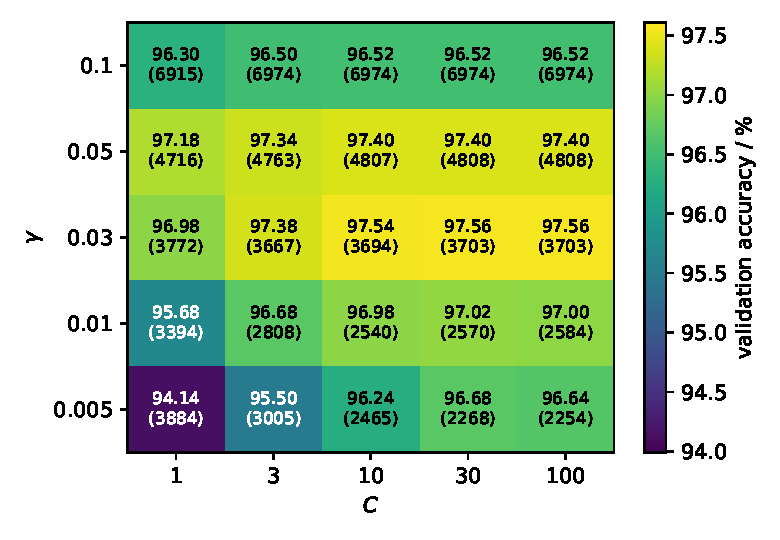
\includegraphics[width=0.62\textwidth]{figures/mnist_rbf_grid.pdf}
  \caption{RBF SVM 网格搜索：$C\times\gamma$ 平面的验证准确率/\%（括号内为支持向量数，PCA50 降维、10000 训练子集）}
  \label{fig:rbf_grid}
\end{figure}

\begin{figure}[H]
  \centering
  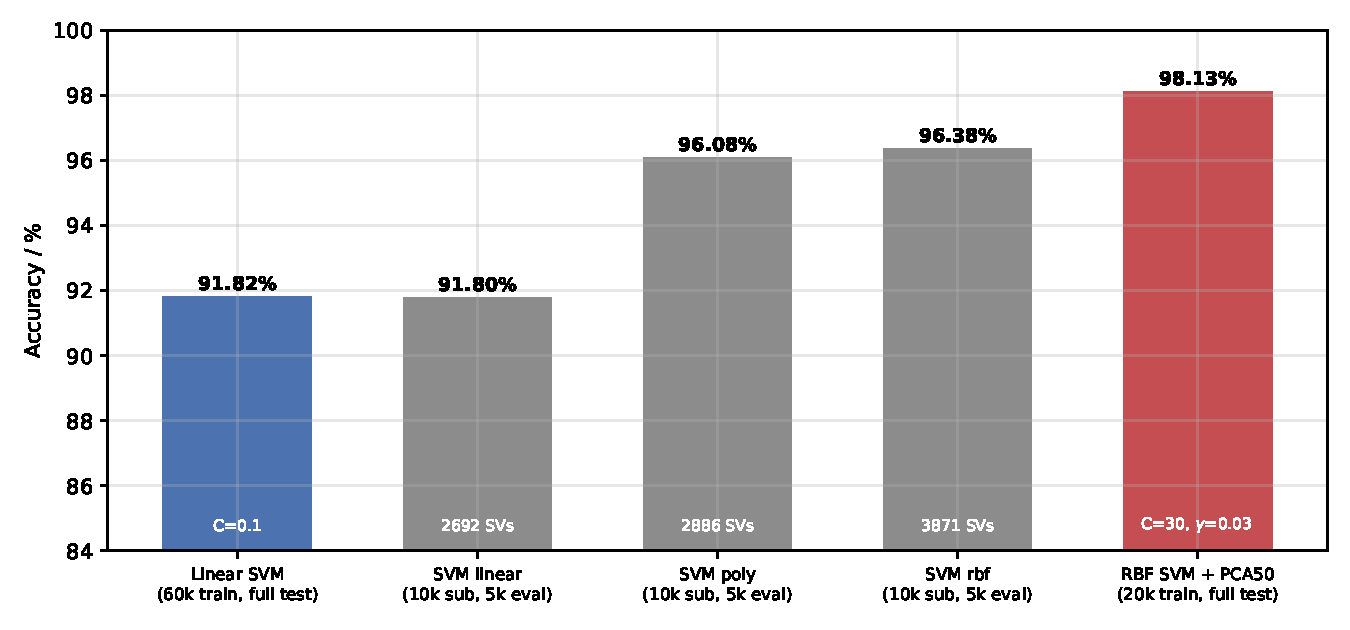
\includegraphics[width=\textwidth]{figures/mnist_svm_comparison.pdf}
  \caption{MNIST 各 SVM 模型准确率对比}
  \label{fig:svm_cmp}
\end{figure}

\begin{figure}[H]
  \centering
  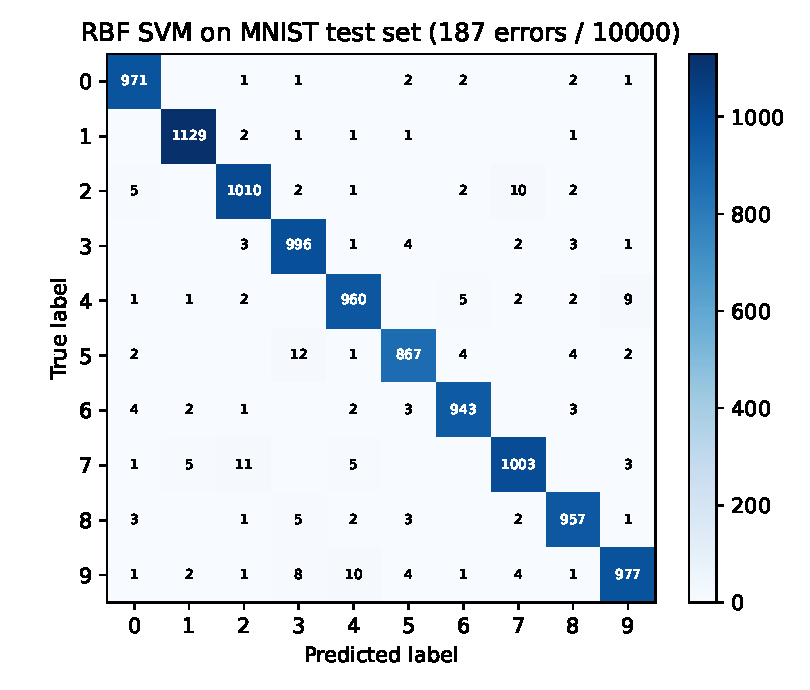
\includegraphics[width=0.56\textwidth]{figures/mnist_svm_confusion_matrix.pdf}
  \caption{RBF SVM（$C=30,\gamma=0.03$，PCA50，20000 训练）的测试集混淆矩阵}
  \label{fig:svm_cm}
\end{figure}

\mlConclusion{1}
结果分析如下：
\begin{enumerate}
  \item 线性 SVM 仅取得 91.82\%，说明 MNIST 在原始像素空间中\textbf{非线性可分}，需要引入非线性；与之对比，同数据下核 SVM（RBF）达到 98.13\%，验证了核技巧在高维特征空间中构造（近似）线性可分表示的有效性；
  \item 核函数对比显示非线性核大幅优于线性核（$+4.6$ 个百分点），且 RBF 略优于多项式核；RBF 的支持向量数（3871/10000）显著多于线性核（2692），说明其决策边界更复杂、更贴合数据分布；
  \item 由图~\ref{fig:rbf_grid} 可见性能对 $\gamma$ 更敏感（每列内准确率差异可达 3 个百分点），$\gamma=0.005$ 时明显欠拟合、$\gamma=0.1$ 时开始过拟合（验证下降且支持向量数激增至约 7000），而 $C$ 增大到一定程度（$\ge 10$）后收益饱和——符合"$C$ 控制正则强度、$\gamma$ 控制模型复杂度量级"的理论预期；
  \item 混淆矩阵（图~\ref{fig:svm_cm}）显示 187 个错误集中在易混数字对 5$\to$3（12 次）、7$\to$2（11 次）、9$\to$4（10 次）、2$\to$7（10 次）、4$\leftrightarrow$9。与作业2的 MLP（98.90\%）和作业1的 CNN（99.66\%）相比，RBF SVM 仅以 6475 个支持向量系数做推理即达 98.13\%，模型紧凑、训练耗时仅约 1 分钟，但准确率低约 0.8--1.5 个百分点，说明对图像数据而言局部卷积结构（权重共享+平移先验）优于通用的像素距离核；
  \item 训练/推理开销随支持向量数线性增长（线性 SVM 测试 0.05~s vs RBF SVM 3.0~s），这是核 SVM 难以直接扩展到完整 60000 样本乃至更大数据集的主要原因，也是实践中采用 PCA 降维与子采样的动因。
\end{enumerate}

\mlExperiment{5.2}{波士顿房价回归：SVR 回归系统}
Baseline 为线性回归；对比线性 SVR（$C\times\varepsilon$ 网格：$C\in\{0.1,1,10,100\}$，$\varepsilon\in\{0.01,0.05,0.1,0.3\}$）与 RBF SVR（再乘 $\gamma\in\{0.01,0.05,0.1,0.5\}$，共 64 组），均以验证集 RMSE 选参。结果见表~\ref{tab:boston} 与图~\ref{fig:boston}、图~\ref{fig:boston_res}。

\begin{table}[H]
  \centering
  \caption{波士顿房价各实验结果对比（与作业2同一切分：train/val/test = 323/80/103；RMSE 与 MAE 单位为千美元）}
  \label{tab:boston}
  \footnotesize
  \begin{tabular}{llccc}
    \toprule
    方法 & 最优超参数 & RMSE$\downarrow$ & MAE$\downarrow$ & $R^2\uparrow$ \\
    \midrule
    线性回归（baseline） & --- & 4.732 & 3.194 & 0.6824 \\
    LinearSVR & $C=10,\ \varepsilon=0.3$ & 4.790 & 2.983 & 0.6746 \\
    SVR-RBF & $C=100,\ \gamma=0.01,\ \varepsilon=0.01$ & \textbf{3.070} & \textbf{2.157} & \textbf{0.8663} \\
    \midrule
    SVR-RBF（5 折交叉验证） & 每折内部重选参 & \multicolumn{2}{c}{$3.497\pm0.638$} & $0.8445\pm0.0662$ \\
    \midrule
    MLPNN 13--64--32--1（作业2） & --- & 2.922 & 2.054 & 0.8789 \\
    \bottomrule
  \end{tabular}
\end{table}

\begin{figure}[H]
  \centering
  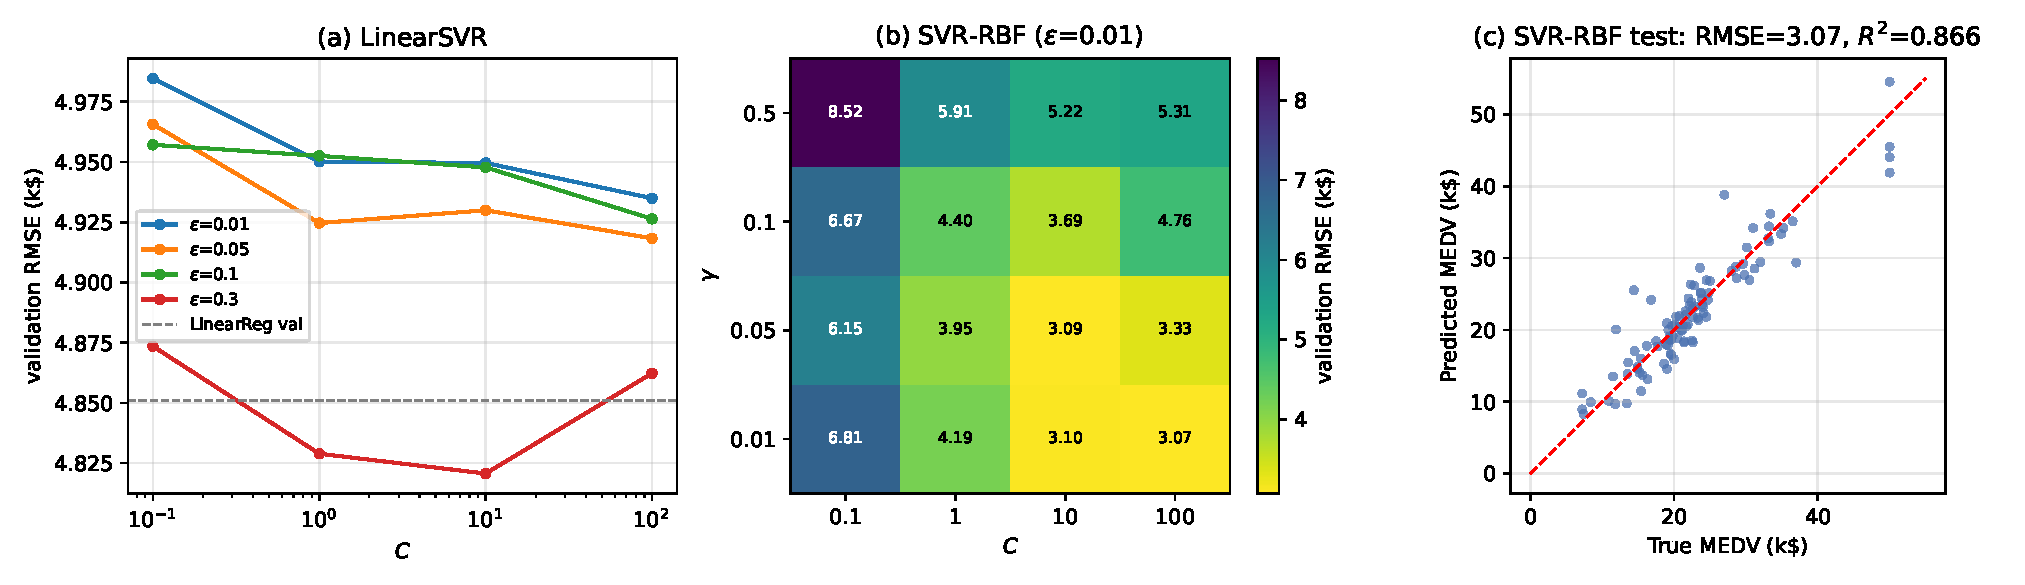
\includegraphics[width=\textwidth]{figures/boston_svr.pdf}
  \caption{(a) LinearSVR 在 $C$ 扫描下不同 $\varepsilon$ 的验证 RMSE（虚线为线性回归验证 RMSE）；(b) SVR-RBF 在最优 $\varepsilon=0.01$ 下 $C\times\gamma$ 平面的验证 RMSE（千美元）；(c) 最优 SVR-RBF 的测试集预测值--真实值散点图}
  \label{fig:boston}
\end{figure}

\begin{figure}[H]
  \centering
  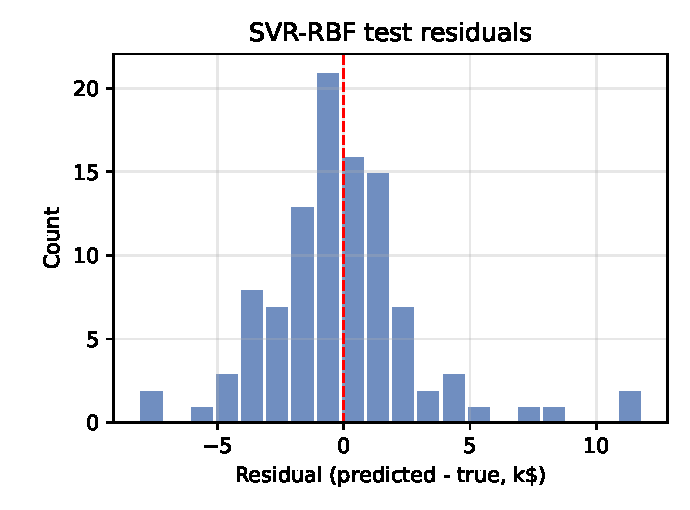
\includegraphics[width=0.5\textwidth]{figures/boston_svr_residuals.pdf}
  \caption{最优 SVR-RBF 的测试集残差直方图（预测值$-$真实值，千美元）}
  \label{fig:boston_res}
\end{figure}

\mlConclusion{2}
结果分析如下：
\begin{enumerate}
  \item LinearSVR（测试 $R^2=0.675$）与线性回归（$R^2=0.682$）几乎持平，说明 $\varepsilon$-不敏感损失本身不提供额外拟合能力，房价数据中的非线性关系必须靠核函数建模；
  \item SVR-RBF 将测试 RMSE 由 4.73 降至 3.07 千美元、$R^2$ 由 0.68 提升至 0.866，显著优于线性模型，接近作业2中最佳 MLPNN 的水平（RMSE 2.92，$R^2$ 0.879），说明 RBF 核对小样本表格数据的非线性拟合能力与深度模型相当；
  \item 由图~\ref{fig:boston}(b) 可见 $C$ 与 $\gamma$ 存在明显交互：$\gamma$ 小（核更"平滑"）时需要较大的 $C$ 才能拟合训练数据；最优模型 323 个训练样本中 316 个成为支持向量，说明目标函数存在不可消除的噪声/异方差，几乎全体样本都落在 $\varepsilon$ 管道之外；
  \item 5 折交叉验证给出 RMSE $=3.50\pm0.64$、$R^2=0.845\pm0.066$，每折自动选出的超参数集中在 $C=10$--$100$、$\gamma\in\{0.01,0.05,0.1\}$，与单次划分结果一致，说明结论稳健，但 506 样本的小数据集上折间波动（标准差 0.64）仍明显大于作业2 MLP 的 CV 结果；
  \item 由图~\ref{fig:boston}(c) 与图~\ref{fig:boston_res} 可见预测点整体紧贴对角线、残差近似以 0 为中心对称分布，但在高价区（MEDV 接近 50 千美元的数据被人为截断）仍有系统性低估，与作业2的观察一致。
\end{enumerate}

\section{总结}
本次作业完整实现了基于 SVM 的分类与回归系统。主要结论：(1) 分类任务中，线性 SVM（91.82\%）无法刻画 MNIST 的非线性结构，RBF 核 SVM 结合 PCA 降维与网格搜索（$C=30,\gamma=0.03$）在 20000 训练子集上达到 98.13\% 测试准确率，核函数与非线性超参数（$\gamma$）是影响性能的首要因素；(2) 回归任务中，RBF SVR（测试 RMSE 3.07 千美元，$R^2=0.866$）显著优于线性模型并与作业2的 MLPNN 接近，5 折交叉验证（RMSE $3.50\pm0.64$）确认结果稳健，$\varepsilon$-不敏感损失与标签标准化、验证集选参是小样本回归的关键；(3) 综合来看，SVM/SVR 在中小规模数据上以极低的训练和调参成本（全部分钟级）取得了与神经网络相当的性能，但其训练复杂度随样本数超线性增长、预测开销随支持向量数增长，面对大规模数据需依赖子采样、降维或近似核方法。后续可尝试 Nystr\"om/RFF 近似核以扩展到完整 MNIST，或在回归任务上引入自动相关确定（ARD）核做特征选择。

\end{document}
